\section{ЧЕТЫРЕХУГОЛЬНИКИ}

\textbf{1847.}

{\centering 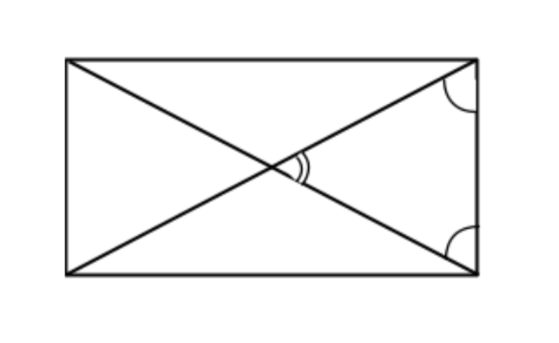
\includegraphics[width=0.5\linewidth]{Geometry/Content/19.png}
	
}
\[
\alpha = 180^\circ - 2\cdot 74^\circ = 32^\circ
\]. \null \hspace*{\fill} Ответ: 32.

\textbf{1848, 1849} - аналогичные задачи.

\textbf{1850.} $\angle ADC = \angle BDA + \angle BDC = 62^\circ + 42^\circ = 104^\circ.$ Т.к. трапеция равнобедренная, то и $\angle BAD = 104^\circ$. Тогда $\angle ABD = 180^\circ -\linebreak- \angle BAD - \angle BDA = 180^\circ - 104^\circ - 62^\circ = 14^\circ.$ \newline \null \hspace*{\fill} Ответ: 14.

\textbf{1851, 1852} - аналогичные задачи.

\textbf{1853.} Если $a$ - сторона квадрата, то его перитметр $P = 4a = 84,$ т.е. $a = 21$. Тогда площадь квадрата 
\[
S = a^2 = 441
\].\null \hspace*{\fill} Ответ: 441.

\textbf{1854, 1855} - аналогичные задачи.

\textbf{1856.} Если расстояние точки пересечения диагоналей от стороны ромба равно 1, то в силу симметрии расстояние равно 1 и до противоположной стороны, так что высота ромба равна 2. Тогда его площадь 
\[
S = ah = 12\cdot 2 = 24
\].\null \hspace*{\fill} Ответ: 24.

\textbf{1857, 1858} - аналогичные задачи.

\textbf{1859.} Поскольку сумма углов, прилежащих к боковой стороне трапеции, равна $180^\circ$, то речь идет о сумме углов, прилежащих к основанию трапеции. Трапеция равнобедренная, поэтому угол при основании равен $\frac{178^\circ}{2} = 89^\circ$. Юольшой угол такой трапеции, очевидно равен $180^\circ - 89^\circ = 91^\circ.$ \newline \null \hspace*{\fill} Ответ: 91.

\textbf{1860, 1861} - аналогичные задачи.

\textbf{1862.} Стороны ромба равны, поэтому одна сторона $a = \frac{P}{2} = \linebreak = \frac{12}{4} = 3$. Тогда площадь ромба $S = a^2\sin{\alpha} = 3^2\cdot\sin{30^\circ} = \linebreak = \frac{9}{2} = 4,5.$ \newline \null \hspace*{\fill} Ответ: 4,5.

\textbf{1863, 1864} - аналогичные задачи.

\textbf{1865.} Из рисунка ясно, что основание параллелограмма $a = \linebreak = 3+ 5 = 8$, а высота $h = 12$. Тогда площадь $S = ah = 8\cdot12=\linebreak=96.$ \newline \null \hspace*{\fill} Ответ: 96.

\textbf{1866, 1867} - аналогичные задачи.

\textbf{1868.}

{\centering 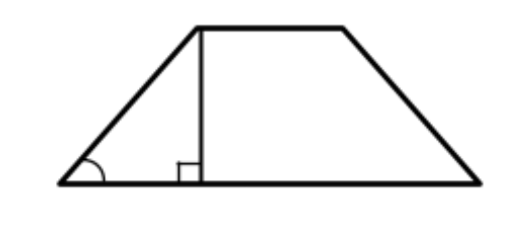
\includegraphics[width=0.5\linewidth]{Geometry/Content/20.png}
	
}

Проведем  высоту $BH \perp AD$.  Поскольку $ABCD$ - равнобедренная трапеция, то в силу симметрии $AH = \frac{AD - BC}{2} = \linebreak = \frac{6 - 2}{2} = 2$. Треугольник $ABH$ - прямоугольный, острый угол равен $45^\circ$, поэтому $h =BH = AH = 2$. Площадь трапеции
\[
S = \frac{a + b}{2}\cdot h=\frac{2 + 6}{2}\cdot 2 = 8
\].\null \hspace*{\fill} Ответ: 8.

\textbf{1869, 1870} - аналогичные задачи. 

\clearpage

\textbf{1971.}

{\centering 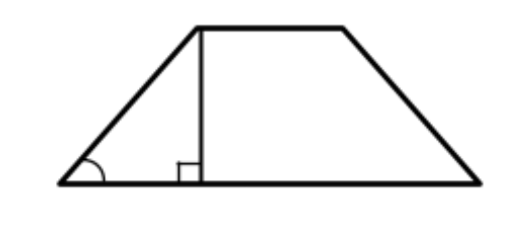
\includegraphics[width=0.5\linewidth]{Geometry/Content/20.png}
	
}

Треугольник $ABH$ - прямоугольный, острый угол равен $45^\circ$, поэтому $AH = BH = 5$. С другой стороны, $ABCD$ - равнобедренная трапеция, тогда в силу симметрии $AH = \frac{b - a}{2}$, где $a$ и $b$ - ее основания. Т.к. $b = 14$, то $a = b - 2AH = 14 - 10 = \linebreak = 4.$. \newline \null \hspace*{\fill} Ответ: 4.

\textbf{1872, 1873} - аналогичные задачи.

\textbf{1874.}

{\centering 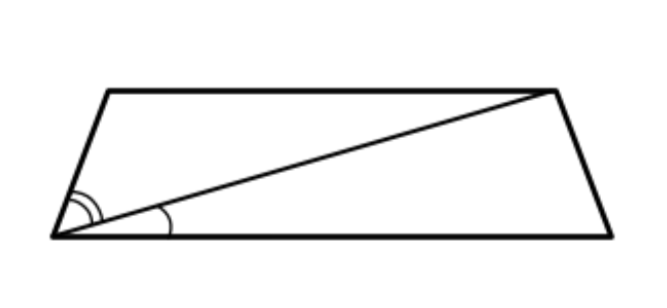
\includegraphics[width=0.5\linewidth]{Geometry/Content/21.png}
	
}
\[
\angle BAD = 54^\circ + 19^\circ = 73^\circ, \;\angle ABC = 180^\circ - 73^\circ = 107^\circ
\].\null \hspace*{\fill} Ответ: 107.

\textbf{1875, 1876} - аналогичные задачи.

\textbf{1877.} $\angle A = 25^\circ + 30^\circ = 55^\circ,$ $\angle D = 180^\circ - \angle A = 125^\circ.$ \newline \null \hspace*{\fill} Ответ: 125.

\textbf{1878, 1879} - аналогичные задачи.

\textbf{1880.}

{\centering 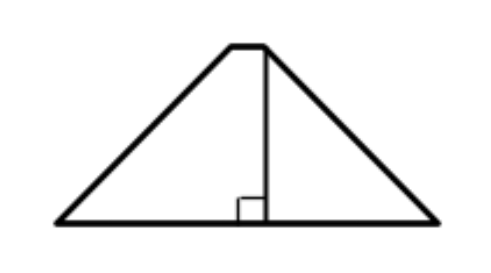
\includegraphics[width=0.4\linewidth]{Geometry/Content/22.png}
	
}
 
 Если $a$ и $b$ - основания равнобедренной трапеции $ABCD$ $(b > a)$, то:
\[
HD = \frac{b - a}{2} = 17,\; AH = b - \frac{b - a}{2} = \frac{b + a}{2} = 19.
\]
Решив систему уравнений  $\begin{cases} b - a =34 \\ b + a = 38 \end{cases}$, найдем значение a = \linebreak = 2. \newline \null \hspace*{\fill} Ответ: 2.

\textbf{1881, 1882} - аналогичные задачи.

\textbf{1883.}

{\centering 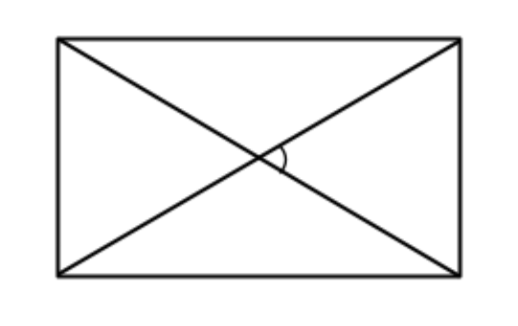
\includegraphics[width=0.5\linewidth]{Geometry/Content/23.png}
	
}

Диагонали прямоугольника равны и в точке пересечения $O$ делятся пополам, а поскольку угол между ними равен $60^\circ$, то   равносторонний, так что $OC = CD = 42,$ $AC= 2OC = 84$. \newline \null \hspace*{\fill} Ответ: 84.

\textbf{1884-1886} - аналогичные задачи.

\textbf{1887.} Пусть $a$ и $a+8$ - стороны параллелограмма. Тогда периметр $P = 2a + 2\cdot(a+8)=100.$
Отсюда $a = 21$. \newline \null \hspace*{\fill} Ответ: 21. 

\textbf{1888-1890} - аналогичные задачи.

\textbf{1891.}

{\centering 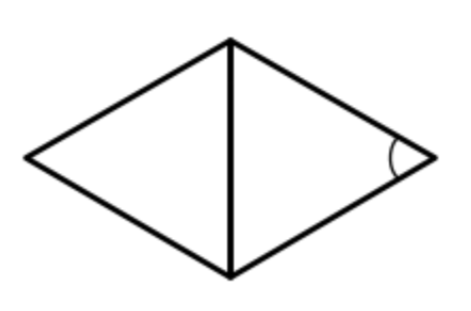
\includegraphics[width=0.4\linewidth]{Geometry/Content/24.png}
	
}

Т.к. стороны ромба равны, а $\angle C = 60^\circ$, то $\Delta BCD$ равносторонний; тогда $BD = DC = 19$. \newline \null \hspace*{\fill} Ответ: 19.  

\textbf{1892-1894} - аналогичные задачи.

\textbf{1895.} Средняя линия трапеции равна полусумме оснований: 
\[\frac{46+66}{2} = 56.\] \null \hspace*{\fill} Ответ: 56.

Из этих же соображений решаются задачи \textbf{1896-1900}.

\textbf{1901.}

{\centering 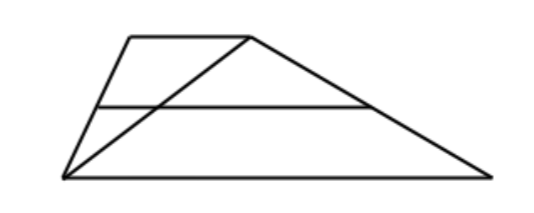
\includegraphics[width=0.5\linewidth]{Geometry/Content/25.png}
	
}

Пусть $ABCD$ - трапеция, $MN$ и $AC$ - ее средняя линия и одна из диагоналей. Отрезки $MO$ и $ON$, на которые делит среднюю линию диагональ, являются средними линиями треугольников $ABCD$ и $ACD$. Поэтому
\[
ON = \frac{AD}{2} = 5
\] \null \hspace*{\fill} Ответ: 5.

\textbf{1902-1904} - аналогичные задачи.

\textbf{1905}. В параллелограмме противоположные углы равны, а прилежащие к одной стороне углы в сумме составляют $180^\circ$; одна пара углов острые, другая - тупые. Если задана сумма углов в $50^\circ$, то это означает, что острый угол равен $\frac{50^\circ}{2} = 25^\circ$. Тогда тупой угол равен $180^\circ - 25^\circ = 155^\circ.$ \newline \null \hspace*{\fill} Ответ: 155.

\textbf{1906-1908} - аналогичные задачи.

\clearpage

\textbf{1909.} В задаче речь идет об углах $\alpha$ и $\beta$, прилежащих к одной стороне. Тогда   $\begin{cases} \alpha - \beta = 52^\circ \\ \alpha + \beta = 180^\circ \end{cases}$. Поэтому $2\alpha = 232,$ $\alpha = 116^\circ.$ \newline \null \hspace*{\fill} Ответ: 116.

\textbf{1910-1912} - аналогичные задачи.

\textbf{1913.} $\begin{cases} \alpha = \frac{31}{5}\beta \\ \alpha + \beta = 180^\circ \end{cases}$. Отсюда $\alpha = 165^\circ.$ \newline \null \hspace*{\fill} Ответ: 165.

\textbf{1914-1916} - аналогичные задачи.

\textbf{1917.}

{\centering 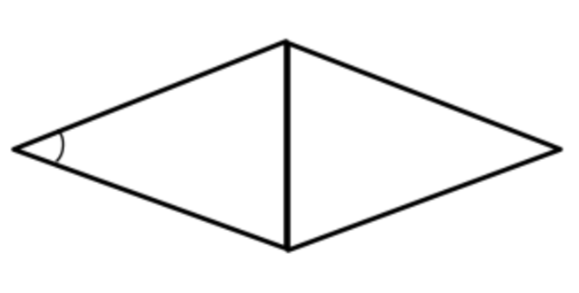
\includegraphics[width=0.4\linewidth]{Geometry/Content/26.png}
	
}

Пусть $ABCD$ - ромб с острым углом $36^\circ$. Тогда его тупой угол $ABC$ равен $180^\circ - 36^\circ = 144^\circ$. Диагональ $BD$ делит этот угол пополам, так что $\angle DBC = 72^\circ.$ \newline \null \hspace*{\fill} Ответ: 72.

Задачи \textbf{1918-1924} решаются по аналогии. 

\textbf{1925.}

{\centering 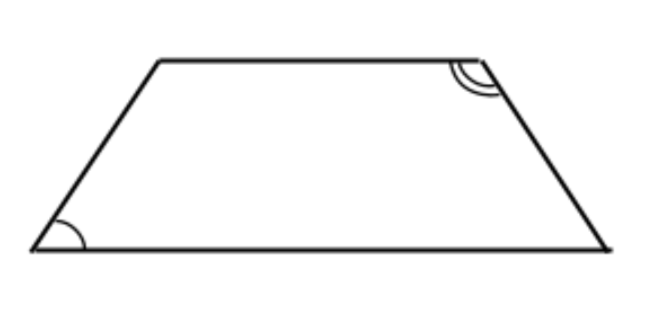
\includegraphics[width=0.5\linewidth]{Geometry/Content/27.png}
	
}

В равнобедренной трапеции сумма противоположных углов составляет $180^\circ$. Поэтому можно записать:
\[
\begin{cases}
	\angle A + \angle C = 180^\circ \\
	\angle C - \angle A = 6^\circ \end{cases}
, \; 2\angle C = 186^\circ, \; \angle C = 93^\circ.\;
\]\null \hspace*{\fill} Ответ: 93.

\textbf{1926-1928} - аналогичные задачи.

\textbf{1929.} $S = \frac{a + b}{2}\cdot h$, $h = \frac{2S}{a + b} = \frac{2\cdot 128}{3 + 13} = 16.$ \newline \null \hspace*{\fill} Ответ: 16.

\textbf{1930-1932} - аналогичные задачи.

\textbf{1933.} $S = \frac{a + b}{2}\cdot h$, $a + b = \frac{2S}{h},$ $a = \frac{2S}{h} - b = \frac{2\cdot 80}{8} - 1 = 19.$ \newline \null \hspace*{\fill} Ответ: 19.

\textbf{1934-1936} - аналогичные задачи.

\textbf{1937.}

{\centering 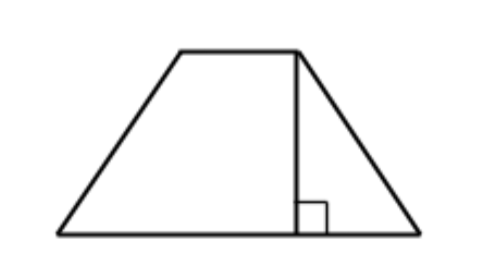
\includegraphics[width=0.45\linewidth]{Geometry/Content/28.png}
	
}

Пусть $BC = a = 4$, $AD = b = 16$ - основания трапеции, $P=40$ и $l$ - ее периметр и боковая сторона. Тогда
\[
CD = l = \frac{P-a-b}{2} = \frac{40-4-16}{2} = 10.
\]
Проведем высоту $CH \perp AD$. В силу симметрии $HD = \frac{b - a}{2} = 6$. Из прямоугольного $\Delta CDH$ найдем высоту трапеции: $CH = h =\linebreak= \sqrt{CD^2-HD^2} = \sqrt{10^2-6^2} = 8$. Площадь трапеции
\[
S = \frac{a+b}{2}\cdot h = \frac{4 + 16}{2} \cdot 8 = 80.
\] \null \hspace*{\fill} Ответ: 80.

\textbf{1938-1940} - аналогичные задачи.

\textbf{1941.}

{\centering 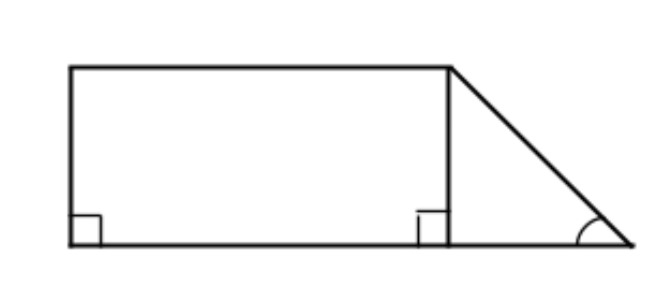
\includegraphics[width=0.45\linewidth]{Geometry/Content/29.png}
	
}

Пусть в трапеции $ABCD$ $\angle A = 90^\circ$, $\angle D = 45^\circ$, $BC = 16,$ $AD = \linebreak=18$. Проведем высоту $CH \perp AD$. Тогда $HD = AD - BC = \linebreak = 2$, а из равнобедренного прямоугольного $\Delta CDH$ $CH = h = \linebreak = HD = 2$. Площадь трапеции
\[
S = \frac{AD + BC}{2}\cdot h = \frac{18+16}{2}\cdot2=34.
\] \null \hspace*{\fill} Ответ: 34.

\textbf{1942-1944} - аналогичные задачи.

\textbf{1945.} Высота трапеции $h = \frac{2S}{a+b} = \frac{2 \cdot 168}{9+18} = 12$. Боковая сторона равнобедренной трапеции
\[
l = \sqrt{h^2+\left( \frac{b-a}{2} \right)^2} = \sqrt{144 + 25} =13
\]  (см. чертеж и пояснения к задаче \textbf{1937})\newline \null \hspace*{\fill} Ответ: 13.

\textbf{1946-1948} - аналогичные задачи.

\textbf{1949.}

{\centering 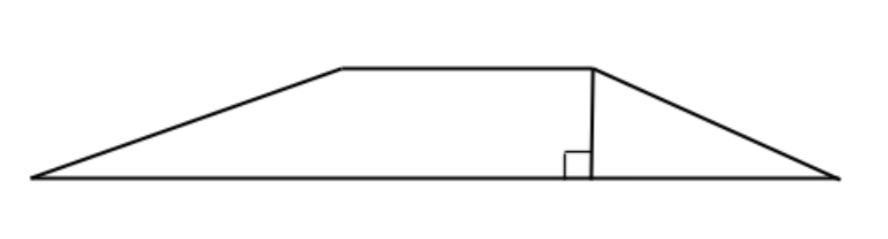
\includegraphics[width=0.6\linewidth]{Geometry/Content/30.png}
	
}

Пусть $ABCD$ трапеция, у которой $BC = 3$, $AD = 15$, $CD = 2$, $\angle BCD = 150^\circ$. Очевидно, что $\angle D = 180^\circ - 150^\circ = 30^\circ$. Проведем высоту $CH \perp AD$. Тогда из прямоугольного $\Delta CHD$ $CH = h= \linebreak = \frac{CD}{2} = 1$. Площадь трапеции
\[
S = \frac{AD+BC}{2}\cdot h = 9.
\] \null \hspace*{\fill} Ответ: 9.

\textbf{1950-1952} - аналогичные задачи.

\textbf{1953.} Пусть $a$ и $b$ - стороны прямоугольника. Условие задачи позволяет записать систему уравнений:
\[
\begin{cases}
	2(a+b)=20 \\
	a-b=8
\end{cases}.
\]
Решив ее, найдем: $a =9$, $b = 1$. Тогда $S = ab = 9.$ \newline \null \hspace*{\fill} Ответ: 9.

\textbf{1954-1956} - аналогичные задачи.

\textbf{1957.} Пусть $3x$ и $20x$ - стороны прямоугольника. Тогда $2\cdot(3x+\linebreak+20x)=46x=92$, откуда $x =2$, а площадь прямоугольника
\[
S = 3x\cdot20x=60x^2=240.
\]
\null \hspace*{\fill} Ответ: 240.

Задачи \textbf{1958-1964} решаются на основании аналогичных рассуждений.

\textbf{1965.} Пусть $x$ и $y$ -  стороны прямоугольника. Из условия задачи следует:
\[
\begin{cases} 
	2(x+y)=24\\
	xy=20
\end{cases},
\begin{cases}
	x+y=12\\
	xy=20
\end{cases}.
\]
В соответствии с теоремой Виета $x$ и $y$ являются корнями квадратного уравнения $t^2-12t+20=0$. Больший корень этого уравнения равен 10. \newline \null \hspace*{\fill} Ответ: 10.

\textbf{1966-1968} - аналогичные задачи.

\textbf{1969.} В прямоугольнике квадрат диагонали равен сумме квадратов двух смежных сторон $x$ и $y$ .  Это позволяет записать следующую систему уравнений:
\[
\begin{cases} 
	2(x+y)=30\\
	x^2+y^2=14^2
\end{cases},
\begin{cases}
	x+y=15\\
	x^2+y^2=196
\end{cases}.
\]
Возведем первое уравнение в квадрат и вычтем из него второе; получим $2xy=225-196$. Отсюда $xy=14,5$, а это и есть площадь прямоугольника. \newline \null \hspace*{\fill} Ответ: 14,5.

\textbf{1970-1972} - аналогичные задачи.

\clearpage 

\textbf{1973.}

{\centering 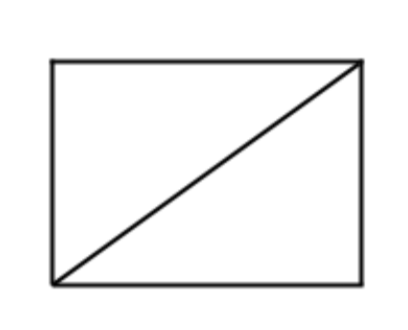
\includegraphics[width=0.4\linewidth]{Geometry/Content/31.png}
	
}

Пусть $AC$ - диагональ прямоугольника, а $CD = 9$ - одна из сторон. Обозначим $AC = 5x$, $AD = 4x$. Т.к. $AC^2 = AD^2 +CD^2$, то
$25x^2 = 16x^2 +81$, т.е. $x^2=9$ и $x =3$. Площадь прямоугольника
\[
S =AD\cdot DC = 12\cdot 9 =108
\]
\null \hspace*{\fill} Ответ: 108.

\textbf{1974-1976} - аналогичные задачи.

\textbf{1977.} Очевидно $44\cdot 66 = 88\cdot h$, где $h$ - высота, опущенная на большую сторону. Поэтому
\[
h = \frac{44\cdot66}{88} = 33.
\]
\null \hspace*{\fill} Ответ: 33.

Аналогично решаются задачи \textbf{1978-1980}.

\textbf{1981.}

{\centering 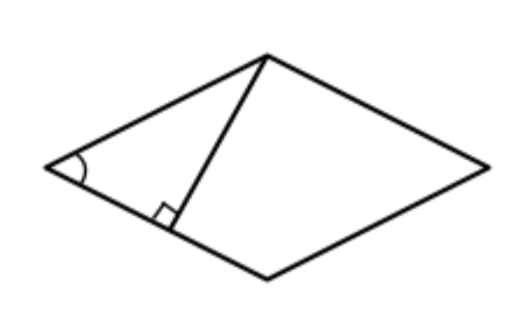
\includegraphics[width=0.45\linewidth]{Geometry/Content/32.png}
	
}

Пусть $BH = h$ - высота ромба. Поскольку в прямоугольном треугольнике $ABH$ эта высота является катетом, лежащим против угла $30^\circ$, сторона ромба $AB$ в два раза больше, т.е. равна 12. Тогда площадь ромба

\[
S = 12 \cdot 6 = 72.
\]
\null \hspace*{\fill} Ответ: 72.

\textbf{1982-1984} - аналогичные задачи.

\textbf{1985.} Площадь ромба равна половине произведения его диагоналей:
\[
S = \frac{13\cdot6}{2}=39.
\]
\null \hspace*{\fill} Ответ: 39.

\textbf{1986-1988} - аналогичные задачи.

\textbf{1989.} Пусть $d_1=x$, $d_2=6x$ - диагонали ромба. Площадь ромба $S = \frac{d_1d_2}{2}=3x^2$. Отсюда $x = \sqrt{\frac{S}{3}} = \sqrt{\frac{48}{3}}=4$. \newline \null \hspace*{\fill} Ответ: 4.

\textbf{1990-1992} - аналогичные задачи.

\textbf{1993.}  Если $d$ - диагональ квадрата, его площадь вычисляется по формуле $S = \frac{d^2}{2}$, поэтому $d = \sqrt{2S} = \sqrt{2\cdot98}=14.$ \newline \null \hspace*{\fill} Ответ: 14.

\textbf{1995, 1996} - аналогичные задачи.

\textbf{1997.} Площадь прямоугольника равна $0,5\cdot2=1$.  Приравнивая ее площади квадрата $a^2$, получаем длину стороны квадрата $a=\linebreak=1$.
\newline \null \hspace*{\fill} Ответ: 1.

Аналогично решаются задачи \textbf{1998-2000}.

\textbf{2001.} $S = ab\sin{\alpha}=12\cdot11\cdot\sin{30^\circ}=66$ \newline \null \hspace*{\fill} Ответ: 66.

\textbf{2002-2004} - аналогичные задачи.

\textbf{2005.} $S = a^2\sin{\alpha}=6^2\cdot\sin{150^\circ}=36\cdot\frac{1}{2}=18$ \newline \null \hspace*{\fill} Ответ: 18.

\textbf{2006-2008} - аналогичные задачи.

\textbf{2009.} $S = \frac{a+b}{2}\cdot h = \frac{36+9}{2}\cdot 2=45.$ \newline \null \hspace*{\fill} Ответ: 45.

\textbf{2010-2012} - аналогичные задачи.

\textbf{2013.} Если линейные размеры сходственных элементов (сторон, биссектрис, медиан, периметров и т.д.) подобных многоугольников относятся как $k$, то площади относятся как квадрат коэффициента подобия $k^2$. Поэтому площадь большего многоугольника равна $9\cdot10^2=900$ \newline \null \hspace*{\fill} Ответ: 900.

\textbf{2014-2016} - аналогичные задачи.